\subsection{Factory Method}
\subsubsection{Địng nghĩa}
Factory Method là một Pattern dùng để cung cấp interface để tạo các objects ở trong super-class, nhưng cho phép các sub-classes quyết định xem loại object nào sẽ được tạo ra.
\subsubsection{Cách sử dụng}
Ta sử dụng factory method trong các trường hợp sau:
\begin{itemize}
    \item Khi bạn muốn tạo một Object mà không cần xác định Object đó thuộc Class nào. Thay vì tạo Object bằng cách gọi trực tiếp từ constructor, bạn sẽ sử dụng một phương thức factory để tạo đối tượng.
    \item Khi bạn muốn có một hệ thống dễ dàng mở rộng bởi vì Factory Method cho phép bạn mở rộng việc tạo các Object bằng cách thêm các SubClass mới mà không làm thay đổi mã nguồn của SuperClass.
    \item Khi bạn muốn áp dụng các kỹ thuật khác nhau để tạo ra Object dựa trên các yêu cầu hoặc tình huống khác nhau. Factory Method cho phép bạn triển khai các phương thức factory khác nhau trong các SubClass để tạo đối tượng theo cách tùy chỉnh.
\end{itemize}
\subsubsection{Cấu trúc}
Factory Method Pattern gợi ý chúng ta thay vì sử dụng phương thức gọi trực tiếp (\textbf{new} operator), chúng ta gọi thông qua một hàm của factory và các hàm này thường trả về loại object. Các thành phần chính của mẫu: \\
\begin{itemize}
    \item Một interface định nghĩa khuôn mẫu cho các sản phẩm được tạo ra.
    \item Các subclass kế thừa từ interface tạo ra hàng loạt loại sản phẩm khác nhau.
    \item Một interface định nghĩa factory method trả về kiểu đối tượng sản phẩm.
    \item Các subclass kế thừa từ interface trên tạo ra hàng loạt class trả về các đối tượng sản phẩm cần.
\end{itemize}
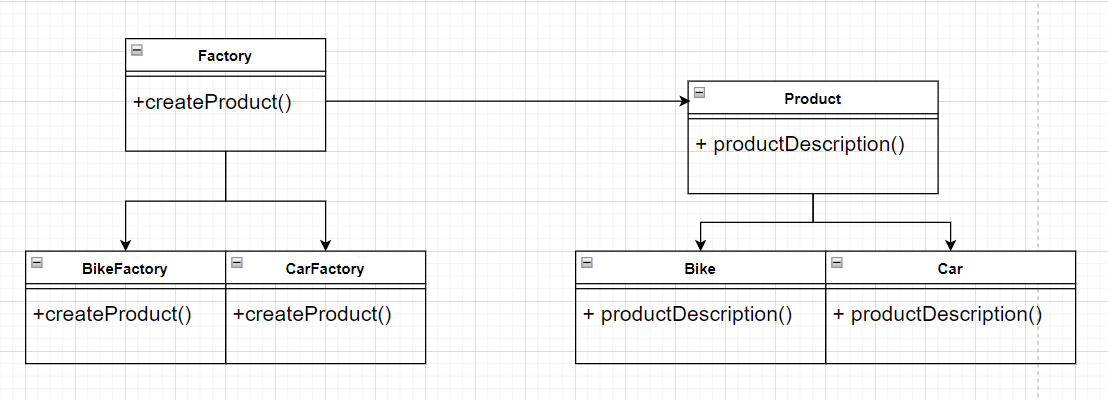
\includegraphics[scale=0.65]{image/creational/cso.png}
\subsubsection{Ưu điểm và Nhược điểm}
Ta thường thấy các ưu nhược điểm sau:\\\\
Ưu điểm:
\begin{itemize}
    \item Tăng tính linh hoạt và tái sử dụng trên nhiều dự án khác nhau, nhiều ngôn ngữ khác nhau.
    \item Dễ dàng mở rộng hay thu hẹp quy mô dự án mà không ảnh hưởng đến các bộ phận khác do các Class khởi tạo không liên quan trực tiếp với nhau.
\end{itemize}
Nhược điểm:
\begin{itemize}
    \item Tăng độ phức tạp: Factory Method có thể làm tăng độ phức tạp của mã nguồn, đặc biệt là khi có nhiều lớp con và các phương thức factory tương ứng.
    \item Nếu không được sử dụng đúng cách, Factory Method có thể dẫn đến việc tạo ra nhiều SubClass thừa thãi không cần thiết.
    \item Khó khăn trong việc theo dõi luồng tạo Object: Khi sử dụng Factory Method, việc theo dõi và hiểu rõ luồng tạo đối tượng có thể trở nên phức tạp khi hệ thống có nhiều SubClass.
\end{itemize}
\subsubsection{Code Example}
Sau đây là code ví dụ mẫu cho Factory Method Pattern có 2 sản phẩm là Bike và Car, cùng với 2 loại Factory là bikeFactory và carFactory. \\
\begin{lstlisting}
#include <iostream>
using namespace std;

class Product
{
public:
    virtual void productDescription() = 0;
};

class Bike : public Product
{
public:
    void productDescription() override { cout << "Bike" << endl; }
};

class Car : public Product
{
public:
    void productDescription() override { cout << "Car" << endl; }
};
//--------------------Factory---------------------
class Factory
{
public:
    virtual Product *createProduct(int n = 0) = 0;
};

class bikeFactory : public Factory
{
public:
    Product *createProduct(int a) override { return new Bike; }
};

class carFactory : public Factory
{
public:
    Product *createProduct(int a) override { return new Car; }
};

int main()
{
    Factory *factory = new bikeFactory();
    factory->createProduct()->productDescription();
    Factory *factory2 = new carFactory();
    factory2->createProduct()->productDescription();
}
\end{lstlisting}
Ở hàm main(), ta tạo 2 nhà máy để sản xuất 2 loại xe khác nhau và cho in ra thông tin 2 loại xe đó.\\
\newline
\textbf{Kết quả:}
\begin{lstlisting}
Bike
Car
\end{lstlisting}
\subsubsection{Các Pattern liên quan}
\begin{itemize}
    \item Thông thường, Factory method hay được sử dụng chung với Abstract Factory Method.
    \item Prototypes: trong một số trường hợp không yêu cầu phân lớp từ Creator. Tu nhiên, chúng thường khởi tạo trên các lớp product.
\end{itemize}